% !TEX root = /Users/Gela/Desktop/Thesis_latex/thesis.tex


\section{Flowchart investigation}
Two different setups for a comparing system to the current system were investigated, section \ref{Flowchart}, and one system, System 2 were chosen to be the comparing system. Both Systems were considered fulfilling most of the requirements, section \ref{framing}, for an updated version. Restrictions on the membrane, such as requirements on no back pressure on the membrane lead to the decision on chosing System 2 as a comparing system. 

The two comparing systems were set to:\\
\begin{figure}[h]
\centering
\begin{minipage}{.5\textwidth}
    \centering
    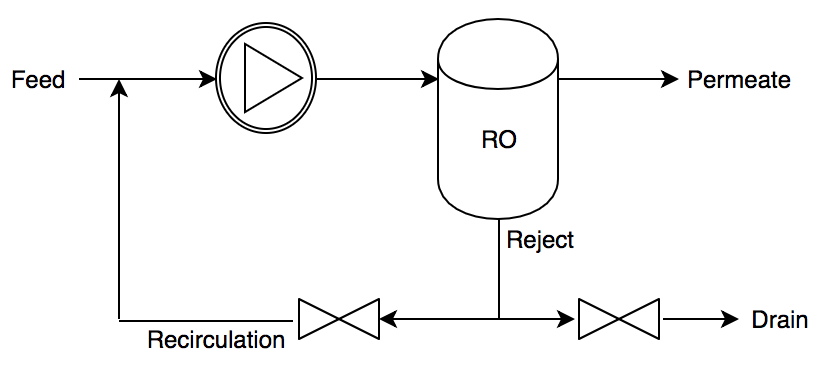
\includegraphics[width=0.8\textwidth]{Sys1}
    \caption{Current System}
    \label{fig:System1}
\end{minipage}%
\begin{minipage}{.5\textwidth}
  \centering
  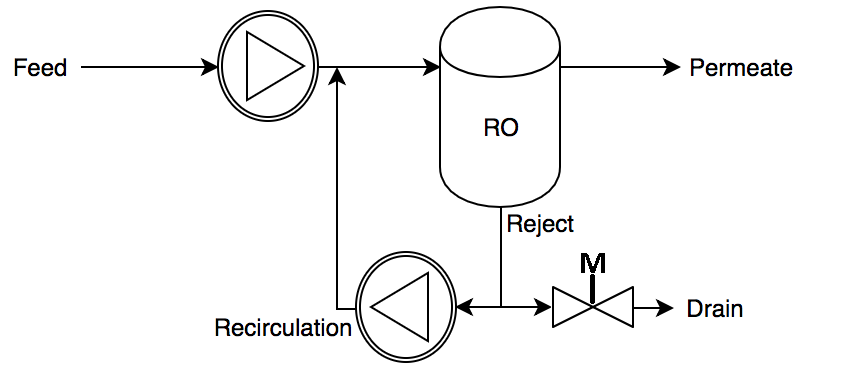
\includegraphics[width=.8\linewidth]{Sys2}
  \caption{System 2}
  \label{fig:System2}
\end{minipage}
\end{figure}

\section{Test on current system}
Results for the test on the current system, figure \ref{fig:Sys1}:

PLOTS FIGURES DATA


\section{Modeling}
A physical model of the membrane were made and the given results were:


FIGURES AND PLOTS FROM SIMSCAPE

\section{Design of control algorithms}

\section{Control simulations}

\section{Implementation test rig}



\section{Improvements}
